\section{Possíveis Soluções}

Existem três principais requisitos de segurança que precisam ser tratado por qualquer projeto de segurança: Confidencialidade, Integridade e Disponibilidade. Confidencialidade garante que apenas o usuário autorizado possa ler o mensagem. A integridade garante que a mensagem enviada seja recebida no destino sem qualquer alteração e disponibilidade significa que cada serviço ou dado esteja disponível para o usuário quando ele necessário. Soluções blockchain são capazes de oferecer esses três requisitos, de maneira bastante eficiente, e por conta disso e da possibilidade de processamento distribuído que blockchain é o tópico estudado nesse artigo como uma possível solução.

\begin{figure}[H]
    \centering
    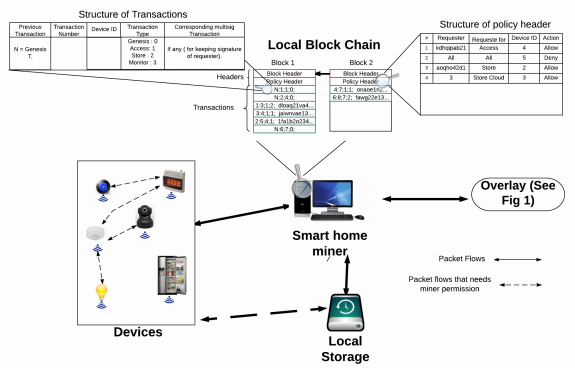
\includegraphics[height=0.5\textwidth]{pictures/home.png}
    \caption{Exemplo de blockchain aplicado em casa inteligente \cite{dorri2017blockchain}}
    \label{fig:home}
\end{figure}

Na figura \ref{fig:home} vemos um exemplo de como blockchain pode ser implementado em uma solução de automação residencial que utiliza IoT. Para aumentar a seguraça da casa inteligente todos os dispositivos conectados a internet estão protegidos contra solicitações maliciosas. Isto é feito limitando as transações aceitas as entidades com as quais cada dispositivo estabeleceu uma chave compartilhada. As transações recebidas da sobreposição são autorizadas antes de encaminhá-las para os dispositivos. Um contra argumento da efetividade dessa estrutura baseada em blockchain é que esse modelo apenas introduz um aumento marginal nos atrasos no processamento de transações em comparação com os produtos de gateway doméstico inteligentes existentes. Há sim também um único atraso adicional durante a inicialização para gerar e distribuir chaves compartilhadas. Em resumo, o adicional atrasos não são significativos e não afetam a disponibilidade de eletrodomésticos inteligentes. Para entender melhor esse modelo, e a forma genérica de como blockchain pode ser implementado em uma rede de qualquer escopo de dispositivos de internet das coisas, vamos separar a implementação em quatro pedaços: transações, blockchain local, minerador e armazenamento local.

As comunicações entre dispositivos locais ou nós de sobreposição são conhecido como transações. Um sistema genérico possui diversas transações, que só podem ser mais especificadas quando saímos do escopo da generalização e entramos no domínio do problema, como é o exemplo da casa inteligente, em que a transação da loja é gerada por dispositivos para armazenar dados, a transação de acesso é gerada por um SP (Service Provider) ou o dono da casa para acessar o armazenamento em nuvem e uma transação de monitor é gerada pelo proprietário da casa ou SPs para monitorar periodicamente um dispositivo em formação. Adicionar um novo dispositivo para a casa inteligente acontece através de uma transação gênesis e um dispositivo é removido através de uma transação de remoção. Todas as transações acima mencionadas usam uma chave compartilhada para proteger a comunicação. Lightweight Hashing é empregado para detectar qualquer alteração no conteúdo das transações durante a transmissão. Todas as transações de ou para a casa inteligente são armazenados em um local privado blockchain. Ou seja, se formos tomar isso em um aspecto genérico, as transações são responsáveis pela comunicação entre os diferentes atores envolvidos, sejam coisas conectadas a internet, um SP, a nuvem ou o usuário.

A blockchain privada local é mantida para acompanhar as transações e tem um cabeçalho de políticas para serem aplicas nos usuários para transações de entrada e saída. Começando com a transação gênesis, as transações de cada dispositivo são encadeadas juntos como um livro de registro imutável na blockchain. Cada bloco na blockchain local contém dois cabeçalhos, o de bloco e o de política. No cabeçalho do bloco tem o hash do bloco anterior para manter o BC imutável. O cabeçalho de política é usado para autorizar dispositivos e impor política de controle do proprietário sobre o sistema em que o blockchain foi aplicado (e.g. o dono da casa). O cabeçalho de política tem quatro parâmetros. O parâmetro ``Requester'' refere-se ao solicitante de chave pública na transação de sobreposição recebida. Para dispositivos locais, este campo é igual ao ``ID do dispositivo''. A segunda coluna no cabeçalho da política indica a ação solicitada na transação, que pode ser: armazenar para armazenar dados localmente, armazenar nuvem para armazenar dados no armazenamento em nuvem, acesso para acessar dados armazenados de um dispositivo e monitorar para acessar dados em tempo real de um dispositivo. A terceira coluna no cabeçalho da política é o ID do dispositivo dentro do sistema e , finalmente, a última coluna indica a ação que deve ser feita para a transação que corresponde com as propriedades anteriores. Além dos cabeçalhos, cada bloco contém um número de transações. Para cada transação, cinco parâmetros são armazenados na blockchain local. Os dois primeiros parâmetros são usados para encadear transações do mesmo dispositivo para o outro e identificar cada transação exclusivamente na blockchain. O ID do dispositivo correspondente da transação é inserido no terceiro campo. ``Tipo de transação'' refere-se a o tipo de transação que pode ser gênese, acesso, armazenamento ou monitorar transações. A transação é armazenada no quinto campo se vem da rede de sobreposição, caso contrário, este campo é mantido em branco. A blockchain local é mantido e gerenciado por um mineirador.

O mineirador do sistema é um dispositivo que processa de maneira centralizar transações de entrada e saída do sistema. O mineirador pode se integrar ao gateway de internet do sistema ou um dispositivo independente separado. O mineirador autentica, autoriza e monitora transações. Além disso, o mineirador também realiza as seguintes funções adicionais: gerar transações de gênese, distrubuição e atualização de chaves, alterar a estrutura de transações e formar e gerenciar o cluster. O minerador coleta todas as transações em um bloco e acrescenta o bloco inteiro ao blockchain. Para fornecer capacidade, o minerador gerencia um armazenamento local.

O armazenamento local é um dispositivo de armazenamento, por exemplo uma unidade de backup, que é usado por dispositivos para armazenar dados localmente. Este armazenamento pode ser integrado com o minerador ou pode ser um dispositivo separado. O armazenamento usa o método FIFO (first-in-first-out) para armazenar dados e armazena os dados de cada dispositivo como um ledger encadeado ao ponto de partida do dispositivo.

Esse é um modelo genérico que é capaz de descrever grande parte das implantações de sistemas blockchain como solução de segurança pra redes de internet das coisas. Outros modelos podem representar de maneira equivalente as características aqui demonstradas, com igual valor semântico.